\section{Introduzione}
\textcolor{blue}{\lipsum[1-2]}

\section{Background}

\begin{figure*}
	\begin{subfigure}{0.6\linewidth}
		\centering
		\footnotesize{ \def\svgwidth{\linewidth}
	    \input{channel_draw.pdf_tex}}
		\caption{}
	\end{subfigure}\hfill
	\begin{subfigure}{0.4\linewidth}
	\centering
	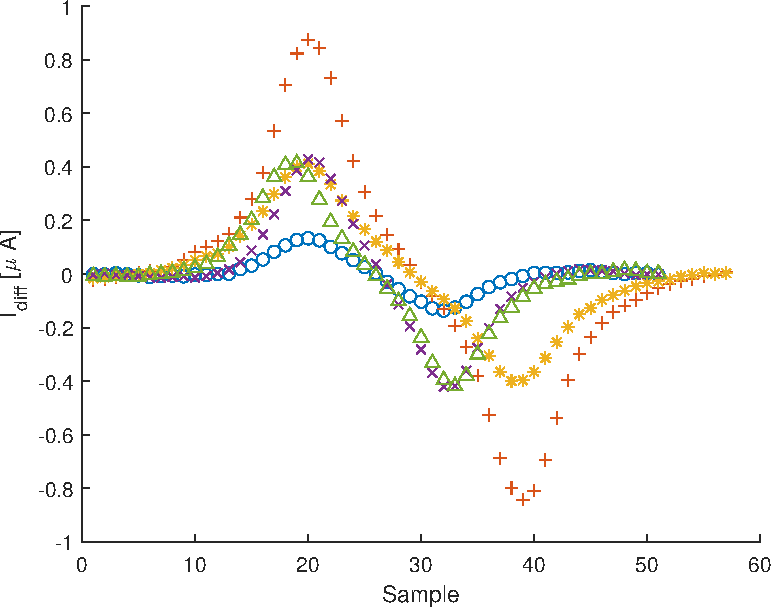
\includegraphics[width=.95\linewidth]{signal_visualization_fig.pdf}
	\caption{}
\end{subfigure}
\caption{}
\label{fig:generale}
\end{figure*}

Il citometro ad impedenza è un dispositivo COMPLETA COMPLETA

Ovvero n on è altro che un microcanale riempito di un buffer conduttivo al cui interno passano delle correnti elettriche. Nel dispositivo in questione si applica un potenziale all'elettrodo centrale e si misura una corrente differenziale tra i due elettrodi laterali.

METTI CREF FIGURA

Tramite la misura di corrente differenziale è possibile stimare alcune proprietà della cellula che passa nel canale. In particolare, al passaggio delle cellula, si misura un segnale con una forma d'onda di tipo gaussiana bipolare.

Tramite il segnale di picco è possibile stimare il diametro. Il segnale è proporzionale al volume della cellula per cui il diametro sarà legato all'ampiezza del segnale ($a$) come:


\begin{equation}
	D=G a^{1 / 3}
\end{equation}

Dove $G$ è un guadagno che risente delle proprietà elettriche del citometro.

\subsection{Gaussiana bipolare}

\begin{figure}
		\centering
		\footnotesize{ \def\svgwidth{0.95\linewidth}
			\input{bipolarGaussian.pdf_tex}}
	\caption{}
	\label{fig:gaussiana}
\end{figure}


La gaussiana bipolare è una forma d'onda caratteristica composta da due gaussiane identificata dalla generica equazione:

\begin{equation}
	g(t)=a\left[e^{g_{+}(t)}-e^{g_{-}(t)}\right]
\end{equation}

Ovvero, considerata un'ampiezza di riferimento $a$ (i.e. il valore massimo di picco), è la somma di due gaussiane nel tempo di cui la seconda ribaltata. La distanza picco-picco è pari a $\delta$ e si introduce un parametro di centratura $t_c$. Le due gaussiane condividono la medesima deviazione standard $\sigma$ e sono identificate dall'equazione:

\begin{equation}
	g_{\pm}(t)=\frac{-\left(t-\left(t_{c} \pm(\delta / 2)\right)\right)^{2}}{2 \sigma^{2}}
\end{equation}

Dove il segno $\pm$ va riferimento alla gaussiana positiva o ribaltata.

\subsection{Procedura di fitting}

Partendo dai dati sperimentali è necessario introdurre una procedura di fitting numerico per identificare la gaussiana, e quindi i suoi quattro parametri descrittivi, tale da rappresentare il segnale analizzato.

Tale procedura di fitting viene implmentata secondo un algoritmo di ottimizzazione. Ovvero, si cerca di ridurre la differenza tra il dato misurato $[d]_i$ e il template di fitting ($g$) allo stesso instante temporale. 

Definita la funzione di errore come tale differenza:

\begin{equation}
	\underline{e}=[d]_{i}-g_{i}\left(t_{i}, a,t_c,\delta,\sigma\right)
\end{equation}

Si cerca di minimizzare la funzione obiettivo definita proprio come la norma dell'errore:

\begin{equation}
	\mathrm{E}(a,t_c,\delta,\sigma) = \frac{1}{2} \sum_{i}\left\|d_{i}-g\left(t_{i},a,t_c,\delta,\sigma\right)\right\|^{2}
\end{equation}


\subsection{Accuratezza}



CITA ERRICO QUI

\section{Risultati}

\subsection{Dataset di riferimento}

Il dataset di riferimento è un insieme di dati grezzi di citometro ad impedenza.  

Per il dispositivo in questione il guadagno è pari a 10.5 $\mu$m / A\textsuperscript{1/3}. I segnali sono campionati con una frequenza $f_s=115$ kHz con un totale di oltre 50.000 segnali.


PARLA DEL DATASET E DEI PARAMETRI 

\subsection{Fitting numerico}



\subsection{Compensazione}


\section{Conclusioni}


%\pagebreak
\section*{Disponibilità dei dati}

Il materiale è disponibile alla repository online del progetto: \url{https://github.com/mastroalex/curve-fitting}


\raggedbottom
%\pagebreak
\printbibliography[title=Riferimenti]
%\section*{References}


\clearpage
\onecolumn
\section*{Appendice}
